%#!lualatex
%#BIBTEX upbibtex jecon-example

%% Filename:            paper.tex
%% Author:              Tomoya Hiroe
%% e-mail               <hiroe-tomoya-yp@ynu.jp>
%% First-written:       <20**/**/**>
%% Description: 
%%
%############################## Main #################################

%% jlreq クラスを利用
\documentclass[article]{jlreq}


\usepackage{fancyhdr}
%% ヘッダー、フッターの設定
\pagestyle{fancy}
    \lhead{} %ヘッダ左
    \chead{} %ヘッダ中央
    \rhead{廣江友哉 2125178} %ヘッダ右.コンパイルした日付を表示
    \lfoot{} %フッタ左
    \cfoot{\thepage} %フッタ中央.ページ番号を表示
    \rfoot{} %フッタ右

% 以下は lualatex 用の設定.
\usepackage[no-math]{fontspec}
\usepackage{luatexja-preset}
\usepackage{luatexja-fontspec}

%% LaTeXやBibTeX関連のロゴ
\usepackage{bxtexlogo}
%% natbib.sty を使う.
\usepackage{natbib}
%% Fancybox
\usepackage{fancybox}
%% For screen command.
\usepackage{ascmac}
%% Font を変更 → Times系に.
\usepackage{newtxtext,newtxmath}

%% 色を付ける.
\usepackage{graphicx}
\usepackage{float}
\usepackage{color}
\definecolor{MyBrown}{rgb}{0.3,0,0}
\definecolor{MyBlue}{rgb}{0,0,0.3}
\definecolor{MyRed}{rgb}{0.6,0,0.1}
\definecolor{MyGreen}{rgb}{0,0.4,0}

%% hyperref
\usepackage[%
bookmarks=true,%
bookmarksnumbered=true,%
colorlinks=true,%
linkcolor=MyBlue,%
citecolor=MyRed,%
filecolor=MyBlue,%
urlcolor=MyGreen%
]{hyperref}

\makeatletter
\ifx\undefined\bysame
\newcommand{\BibTeX}{\textrm{B\kern-.05em\textsc{i\kern-.025em b}\kern-.08em%
T\kern-.1667em\lower.7ex\hbox{E}\kern-.125emX}}
\fi
\ifx\undefined\bysame
\newcommand{\bysameline}{\hskip.3em \leavevmode\rule[.5ex]{3em}{.3pt}\hskip0.5em}
\fi
\makeatother

\setlength{\leftmarginii}{1cm}  
\jlreqsetup{
  itemization_label_length={1\zw, i=1\zw},
  itemization_labelsep={1\zw},  
}

\setlength{\leftmargini}{2\zw}% 2+0.5
\setlength{\leftmarginii}{2\zw}% 1+0.5

\newcommand{\midashi}[1]{\noindent \textbf{#1}}
\newcommand{\midashii}[1]{\noindent \textbf{[#1]}}
\newcommand{\midashiii}[1]{\noindent \textbf{□ #1}}


%%% title, author, acknowledgement, and date
\title{統計・機械学習モデル宿題1}

\author{廣江友哉\;2125178\thanks{Email: \texttt{\href{hiroe-tomoya-yp@ynu.jp}{hiroe-tomoya-yp@ynu.jp}}}}

% \date{2017年11月13日}
\date{\today}

%#####################################################################
%######################### Document Starts ###########################
%#####################################################################
\begin{document}

%%% タイトル付ける.
\maketitle

%%% 目次を出力
\tableofcontents

%########################## Text Starts ##############################


\section{課題1}

\begin{figure}[H]
  \centering
  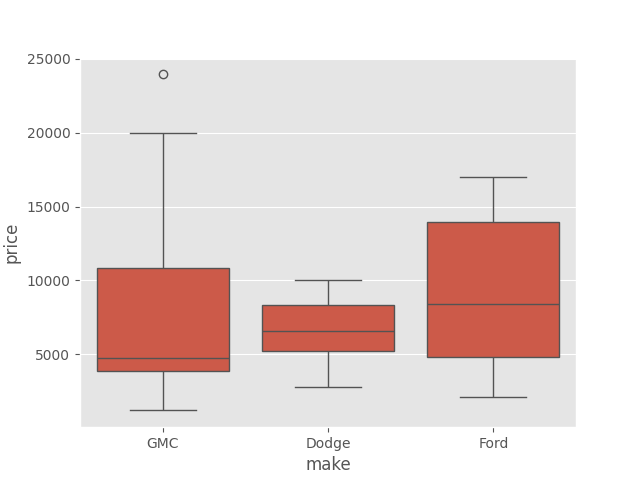
\includegraphics[width=100mm]{../plots/hw1/boxplot.png}
  \caption{箱ひげ図}
\end{figure}

箱ひげ図からメーカーにより価格帯の広がりに違いがあることがわかる.例えば,最低価格と最高価格のトラックのメーカーは共にGMC社である.また,製品価格の中央値が最も小さいのもGMC社である.ここからGMC社は製品価格の分散が他社と比較して大きいことがわかる.一方で,価格の広がりが最も小さいのはDodge社である.四分位範囲も狭く,最高価格は他社と比較して安く,最低価格も他社と比較して高いことがわかる.Ford社は価格の中央値が3社の中で最も高い.

\begin{figure}[H]
  \centering
  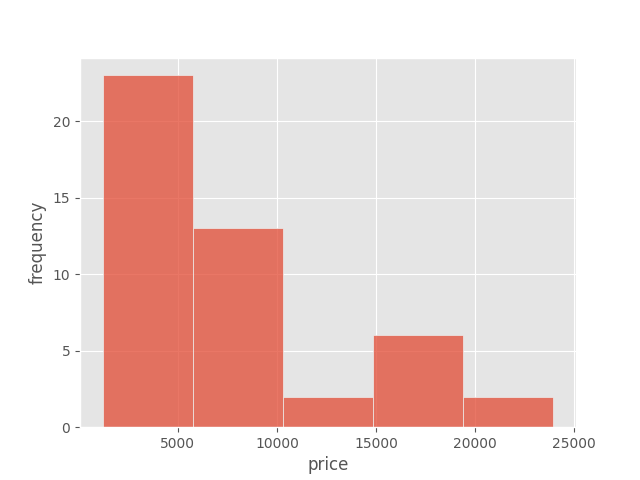
\includegraphics[width=100mm]{../plots/hw1/histogram.png}
  \caption{ヒストグラム}
\end{figure}

図2のヒストグラムは,価格を5つの階級に分けて,0ドル以上25000ドル未満の範囲でプロットしている.0ドル以上5000ドル未満の階級の度数が最も高く,19台である.元のデータは46行からなるCSVデータであるから,中央値が5000ドル以上10000ドル未満の階級に属していることがわかる.

\begin{figure}[H]
  \centering
  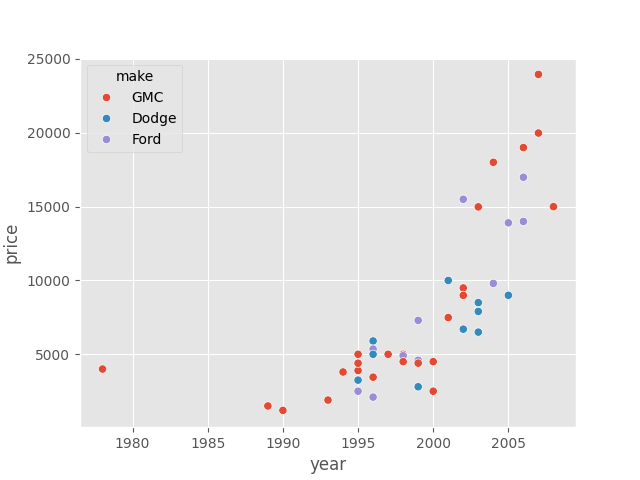
\includegraphics[width=100mm]{../plots/hw1/scatterplot.png}
  \caption{散布図}
\end{figure}

図3の散布図を確認すると,年々トラックの製品価格が高くなる傾向が3社ともに見て取れる.また,図1の箱ひげ図でも確認したように,GMC社の製品には3社の中で最低価格のものと最高価格のものが存在する.さらに,年代に注目すると,最も古いトラックはGMC社のもので,Ford社とDodge社が同時期からデータとして存在することがわかる.

\section{課題2}

\begin{figure}[H]
  \centering
  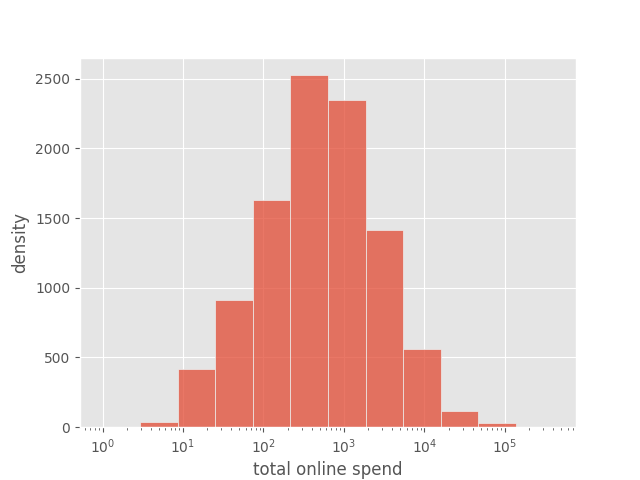
\includegraphics[width=100mm]{../plots/hw1/density.png}
  \caption{ヒストグラム}
\end{figure}

図4のヒストグラムは,オンライン消費額の度数分布を表している.横軸は対数メモリのため,0ドルから10万ドルまでの間に12の階級がある.最も度数の高い階級は,だいたい200ドルから600ドルの間にある階級で2500となっている.

Pythonファイルは完全に動くものを提出するという規則があるため,データはGitHubにgetリクエストを送る形で取得している.また,課題3ではKaggleのデータセットを使用したため,kagglehubというデータセットをインポートするためのライブラリを使用している.また,提出できるファイルにも規則があるため,requirements.txtの代わりにPythonファイルのはじめに必要なライブラリとバージョンをコメントしている.

\section{課題3}


\begin{figure}[H]
  \centering
  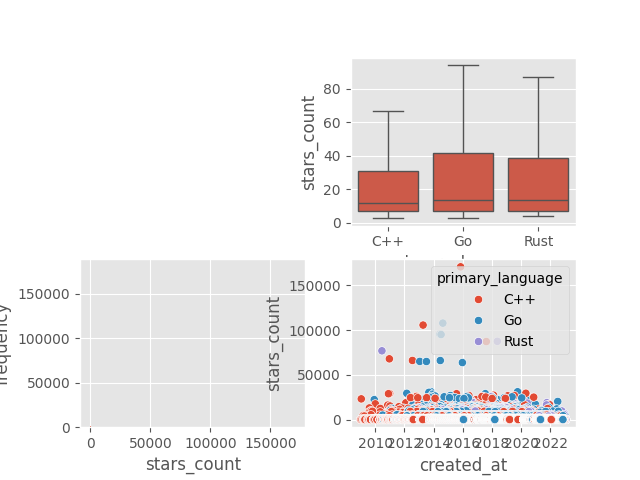
\includegraphics[width=160mm]{../plots/hw1/github.png}
  \caption{Kaggle GitHub datasetのグラフ}
\end{figure}

データはKaggle上で公開されていたGitHub Dataset\footnote{https://www.kaggle.com/datasets/nikhil25803/github-dataset?select=repository\_data.csv}を使用した.このデータセットを選んだ理由は,近年コミュニティの盛り上がりを見せているGo言語,Rust言語,と比較して古典的なプログラミング言語であるC++言語のGitHub上で公開されているリポジトリの中での使用状況を確認するためである.データセットには,レポジトリ\footnote{レポジトリとはGitHub上でコードを扱う際のフォルダのようなもの.例えば,ライブラリのコードは基本的に一つのレポジトリ内に格納される.}毎のデータが行単位で格納されており,レポジトリ名,プルリクエスト\footnote{共同開発のために存在するGitHubの機能.コードに変更を加えたいものがリクエストを作成し,レビュワーがその変更を確認する.プルリクエストの回数はコードの変更回数の目安となる.}の回数,そのレポジトリで使用されている主なプログラミング言語,スター数\footnote{GitHubのお気に入り機能のようなもの.}などのカラムが存在する.

まず,3言語とも外れ値が大きくグラフから関係が読み取りづらい為,箱ひげ図に関しては外れ値を非表示とし,ヒストグラムはx軸を対数目盛りにし,散布図に関しては両軸とも対数目盛りでプロットした.

箱ひげ図では言語毎のスター数をプロットした.外れ値は表示していない.四分位範囲はGo言語が最も広く,中央値もGo言語が一番高いことがわかる.ヒストグラムもスター数を80の階級に分けて表示している.横軸が対数目盛りなのにも関わらず分布が左に寄っている.最も度数が高いのはスター数が4から5の階級であり,約18000のリポジトリがこの階級に属している.したがって,ほとんどのレポジトリのスター数が1ケタから2ケタの間に収まっていることがわかる.特に4ケタを超えるスター数を持つレポジトリはわずかしかないことがわかる.最後に両軸を対数目盛で表示した散布図を確認する.横軸はプルリクエストの回数,縦軸はスター数である.プルリクエストの回数が多いと言うことはそれだけ開発が行われていることを意味するので,開発が行われるだけの需要がありスター数も比例して大きくなると予想していたが,プロットした点は満遍なく広がっており,あまり傾向がみられない.

\bibliographystyle{./jecon}
% \bibliographystyle{./jecon}
% \bibliographystyle{jecon-new}

%% BibTeX データベースファイルの指定.
%
% \addcontentsline{toc}{section}{参考文献}
% \bibliography{./jecon-example}

\end{document}
%#####################################################################
%######################### Document Ends #############################
%#####################################################################
% --------------------
% Local Variables:
% fill-column: 80
% End:
